\chapter{Diagnostic Models}

The last part of this book is about production nodes. Production nodes are where the \textit{magic} happens: they add value to raw materials by transforming them to semifinished or finished products. \par

Here we encounter the highest degree of complexity with low standardisation of the methods, technologies and processes. Nevertheless, it is not a good reason to abandon a data-driven approach.  On the contrary, it is the field where decision-makers benefit the most from this approach linking the model-driven and the data-driven approaches.\par

This chapter focuses on the definition of the keywords and key entities extending the ontology of chapter \ref{chap_InformationFramework} to production nodes. After that, it introduces the diagnostic framework for production nodes with a relational data structure and some KPIs. It will be necessary to pay special attention to the definition of the data structure since it needs the flexibility to host data from very diverse production systems. The same rationale applies to the KPIs where the main KPIs are developed from chapter \ref{chap_InformationFramework}, and applicable to any industries. A smaller subset is, then, introduced to be industry-oriented.\par

Chapter \ref{chapProdControl} focuses on the control of a production node by using analytics to get knowledge on the existing processes and to improve their efficiency. Chapter \ref{chapProdPlantDesign} studies the design of a production facility, and chapter \ref{chapProdProcessDesign} the design of production processes from a data- and model-driven approach.

\section{Ontology}
Here we develop the general ontology introduced in chapter \ref{chap_InformationFramework}, by applying it to a production node. 

\subsubsection{Entities}
We identify the following entities.\par
\textbf{Part} ($i$): It is a piece of raw material, component, subassembly or assembly. Where:
\begin{itemize}
    \item Raw material is a part purchased out of the production node (i.e. from the suppliers).
    \item Component is an individual piece assembled into more complex products.
    \item Subassembly is an assembled unit further assembled into more complex products.
    \item Assembly/final assembly/finished product is the fully assembled product, i.e. the outcome of the production node.
\end{itemize}
\par

\textbf{Processing node} ($j$):A processing node is a resource within the production nodes (e.g. machines and workbenches). In this section, they are also called resources or machines. \par

\textbf{Edge} ($j,k$): The paths connecting resources (e.g. conveyors, corridors) \par

\textbf{Vehicle} ($v$): Is a unit travelling on edges to handle materials between resources; some examples are forklifts, AGVs and conveyors. \par

\textbf{Consumable} ($s$): It is an additional material (often a fluid) or a service necessary to perform activities within the production node. Some examples are electricity, compressed air or steam. \par

\textbf{Route} ($e$): It is the production cycle of a part $i$, i.e. the sequence (ordered set) of resources (machines or workbenches) to visit to transform it to a finished product. \par

\textbf{Order} ($o$): It is a production order received from a customer. \par

\textbf{Job} ($b$): It is a planned activity (a sequence of tasks) to perform on a part $i$ using resources $j$. \par

\textbf{System network} The graph $G(V,A)$ of nodes $j\in V$ and edges $\left(j,k\right)\in A$ composing a Job-shop, flow-shop or a production line.

\subsubsection{Metrics}
We identify the following metrics to assess the performances of a processing node $j$.\par

\textbf{Throughput} ($TH_{j}$): The throughput is the productivity of a resource, i.e. the average number of parts in output per unit of time (e.g., parts produced per hour)..\par

\textbf{Work in process} ($WIP_{j}$): It is the number of parts (i.e., the level of inventory) waiting for processing nearby a resource $j$.\par

\textbf{Work in process} ($WIP_{jk}$): It is the number of parts being transported by a vehicle $v$. \par

\textbf{Capacity} ($C_j$): It is the upper bound of the throughput of a resource.\par

\textbf{Capacity} ($C_v$): It is the maximum number of part transportable by a vehicle $v$ at the same time. \par

\textbf{Utilisation} ($U_j$): It is the average fraction of time that a resource is not idle for lack of parts. \par

\textbf{Utilisation} ($U_v$): It is the average fraction of non-empty space on a vehicle. \par

\textbf{Lead time} ($LT_e$): It is the time allocated for a given route (i.e. to complete the production cycle of a part). \par

\textbf{Cycle time} ($CT_e$): It is the average time from the release of a job to the end of its route. \par

\textbf{Service level} ($SL_e$): $Prob\{cycle\ time\le lead\ time\}$

\subsubsection{Information functions}

Finally, we define the three information functions: Movements $M$ are referred to load/unload of parts on resources; inventories $I$ are referred to the work in process on a resource $j$, or a vehicle $v$. The productivity $P$ refers to the inbound and outbound absorption rates of a resource. Since production resources do not have a decoupling purpose (as, for example, storage system does) it is possible to refer to $P_j=P^{IN}=P^{OUT}$. Table \ref{tab_information_framework_prod} summarises the definition of the three functions in a storage system.

% INSERT tab_information_framework_prod
\begin{figure}[hbt!]
\centering
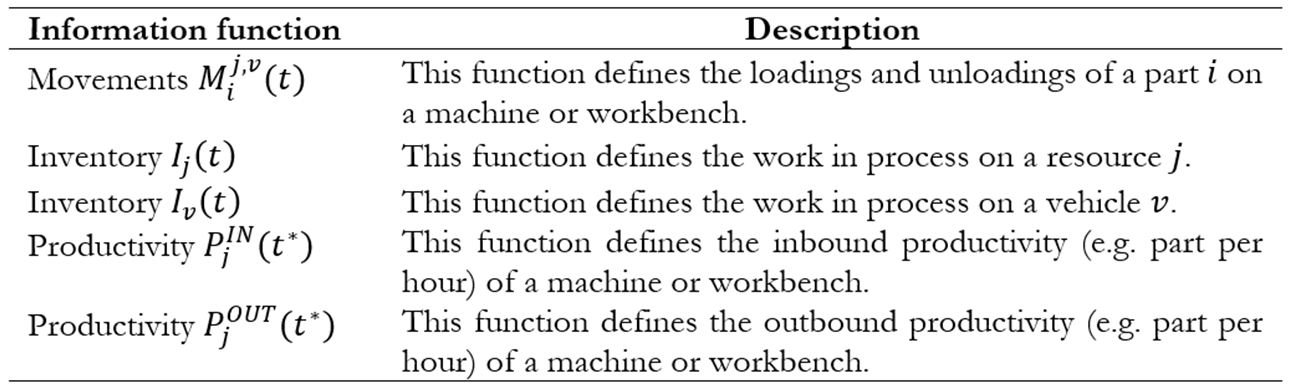
\includegraphics[width=1\textwidth]{sectionProduction/diagnosticModels_figures/tab_information_framework_prod.png}
\captionsetup{type=table}
\caption{Definition of the information functions of a production node.}
\label{tab_information_framework_prod}
\end{figure}


\section{Data Structure} \label{secDataStructureProduction}
Production environments are extremely biased. This paragraph aims at providing data structures that are robust and adaptable to many different production environments. Non-relational structures have this characteristic. For the sake of completeness, this paragraph analyses a traditional relational data structure first. The criticalities of this structure are, then, identified moving to the definition of a non-relational model.

\subsection{A relational model for production environments} \label{secRelationalModelProduction}
Modelling a system with an ER structure means identifying the physical entities with their attributes and the relationship among them. The relationships between entities lead to extraordinarily rigid and instance-oriented data structures which are hardly generalisable in production systems. For this reason, the ER model could not be the best choice to build a model usable for analytics and data-driven modelling, at least not in the case of a production node. We support this fact by empirical evidence starting from the design of an ER model to structure data from the food industry and showing that the model is too rigid to host information from other types of industries. We introduce, then a non-relational model for a production environment with all the ingredients to enable data-driven generalizable models.\par

Modelling is performed by using a top-down approach, starting with the definition of macro-areas that involve similar entities. Afterwards, it is necessary to identify each table (i.e. entities and relations) and the attributes for each table. Following this direction, we apply a top-down approach to a production environment of a food catering industry, identifying three macro-areas to model:

\begin{enumerate}
    \item Supply chain network;
    \item Production plant;
    \item Product quality and control.
\end{enumerate}

Within each of these macro-areas, we identify a set of entities to model using tables.

\subsubsection{Supply chain network}
This macro area considers all the entities linked to the operations performed out of the production plant, which may affect the operations within the production plant. It is the case of customers, suppliers, carriers and other stakeholders connected with the production plant.

\paragraph{Customers-based tables}
These tables deal with distribution flows between production nodes final customer. A table \textit{Nodes} collects the information of the plants involved as producers or suppliers. The attributes of this table are the address, latitude and longitude, working days.  A table \textit{Client} stores similar information for the customers: address, latitude and longitude and the client’s profile (depending on the product/service customisation). A table \textit{Tour} includes the information on the shipping tours. Each tour is performed at a different frequency with a due date for its departure. This time profoundly affects the operations in production since everything must be completed and ready before that time. Besides, each tour has delivery time windows to respect for each client. A relationship between \textit{Tour} and \textit{Client} maps this information.

\paragraph{Demand-based tables}
The table \textit{Orderlist} collects all the information on the customers' order that a production plant needs to process. This table maps the order code, the quantity for each item, the customer, and the service level (i.e. the due time) to deliver the finished product.

\subsubsection{Production plant}
Within this macro-area, we model all the entities involved in the realisation of the final product within the production plant.

\paragraph{Resource-based tables}
These tables map the production resources with their attributes and relationships. A table \textit{Machine category} identifies the different technological group of the machines in the production plant (e.g. lathe, mill, oven). A table \textit{Machine park} identifies all the different variants of the resources in the production area. This table has attributes to record all the specifics of a resource (name, manufacturer, speed, performance, capacity, energy absorption, etc.). \par

The relationship between \textit{Machine category} and \textit{Machine park} defines the type of capacity of the machine too. Especially while dealing with the design of the number of resources, it is necessary to identify a proper measure of capacity. Unfortunately, many different ways exist to define the capacity of a machine. Here we identified the five different types of capacity specifying the units of measure. A machine belongs to one of these types:

\begin{enumerate}
    \item type 1: is a capacity measured with a continuous size metric (e.g. kg or litres);
    \item type 2: is applied to measure the capacity of a machine which has a discrete number of available slots to process parts. Each slot is available/occupied and can host a single part $i$;
    \item type 3 is applied to bottleneck machines that have a throughput metric of capacity. This capacity is measured in a metric belonging to type 1 or type 2 over a time unit (e.g. Kg/h or parts/h);
    \item type 4 is used for buffer and stock areas whose capacity is expressed in cube meters of inventory;
    \item type 5 is used for machines which process entities containing a set of parts (e,g, a tray). Their capacity is expressed in terms of container entities (e.g. number of trays).
\end{enumerate}

A table \textit{Tasks} identifies all the possible activities executable by the resources on the plant layout. Attributes of this table map if a task needs energy to be executed and/or the supervision of a human.

\paragraph{Plant Layout-based tables}
These tables model the placement of the resources on the layout of a production plant. A table \textit{Departments} identifies all the departments of the production area. A table \textit{Control points} identify a set of known coordinates ($x;y;z$) on the plant layout assigning each of them to a department. A table \textit{Machine cp assignment} links a resource from the table \textit{Machine park} to a control point modelling the physical position of a resource on the plant-layout.\par
A table \textit{Machine cycle assignment} defines the relationship between the resources and the production tasks specifying which resource can perform a task.

\paragraph{Auxiliary systems-based table}
These tables identify all the entities (e.g. packages, consumables, energy) which are necessary to perform production tasks. A table \textit{Packages} maps all the packages (e.g. cartons, trays) with their dimensions (i.e. height, length, width) used in the production plant to handle semifinished and finished products. A table \textit{Vehicles} identify all the resource used for the handling of products and packages in the production area. A table \textit{Energy cost} identify the cost for each source of energy of the production plant. A table \textit{Efficiency parameters} identify the behaviour of each machine supplied with a specific source of energy. In particular, for each machine and source of energy, a curve of efficiency is defined as a function of the working time.

\subsubsection{Product, quality and control}
These tables revolve around the product mapping all the information on the product itself (i.e. the bill of materials), the production cycle to realise it, the packaging cycles to pack and customise it and the safety constraints (e.g. temperature and quality decay) associated with the finished product.

\paragraph{Product-based tables}
A table \textit{Products} map all the products identifying their characteristics (e.g., length, width, height, weight, volume), product family and other attributes as:

\begin{itemize}
    \item the slicing profile (mono/multi-portion);
    \item the temperature profile (cook-warm/cook-chill);
    \item the organic profile (organic/non-organic);
    \item the post-processing (eventually mixed after cooking);
    \item the shelflife (in hours or days);
    \item the nutritional values (energy, carbs, fats, protein). 

\end{itemize}

A table \textit{Bill of materials} defines, for each product, the graph where raw materials converge into semi-finished and finished products. The table defines the nodes and edges of the graph specifying which quantity of raw material is necessary to assemble the following semifinished. A table \textit{Cycles} identify the production cycle to transform raw materials into the finished products. Each cycle row defines:

\begin{itemize}
    \item the type of the task;
    \item the quantity of the raw materials (which must be coherent with a machine type capacity);
    \item the working time;
    \item the time type;
    \item the department where the task must be performed;
    \item the temperature-humidity profile.  
\end{itemize}

The working time indicates the time required to perform a specific task, but the real duration of the task depends on the time type. Time type '0' indicates handling activities: the processing time depends on the distance travelled between control points. Time type '1' is a fixed time, not dependent by the processing quantity (e.g. a machine setup). Time type '2' represents cooking time; this time is not conditioned by the quantity but can be affected by temperature and humidity. Time type '3' models a manual operation which depends on the processed quantity. This dependence is hardly linear: less than linear (e.g. logarithmic) curves have been used to estimate the duration of the task. \par
A table \textit{Packaging cycles} defines all the options to package a finished product by identifying the type of packaging and thermal treatment to perform after cooking.

\paragraph{Quality- and control-based tables}
These tables are needed to monitor the quality of the products from the safety point of view that is mainly represented by the temperature in the food industry. A table \textit{Product category} identifies the different thermal category (e.g. cook-chill, cook-warm) of the products and a safe holding temperature for each category. A table \textit{Cycles temperature} collects time-series information from sensors monitoring the temperature and humidity of the products at different stages of the production process.\par

The paragraphs above give a clear picture of the entities and relationship of a food catering plant. The same structure is reported in Figure \ref{fig_prod_er_diagram} illustrating the resulting ER-model. 

% INSERT fig_prod_er_diagram
\begin{landscape}
\thispagestyle{empty}
\begin{figure}[hbt!]
\centering
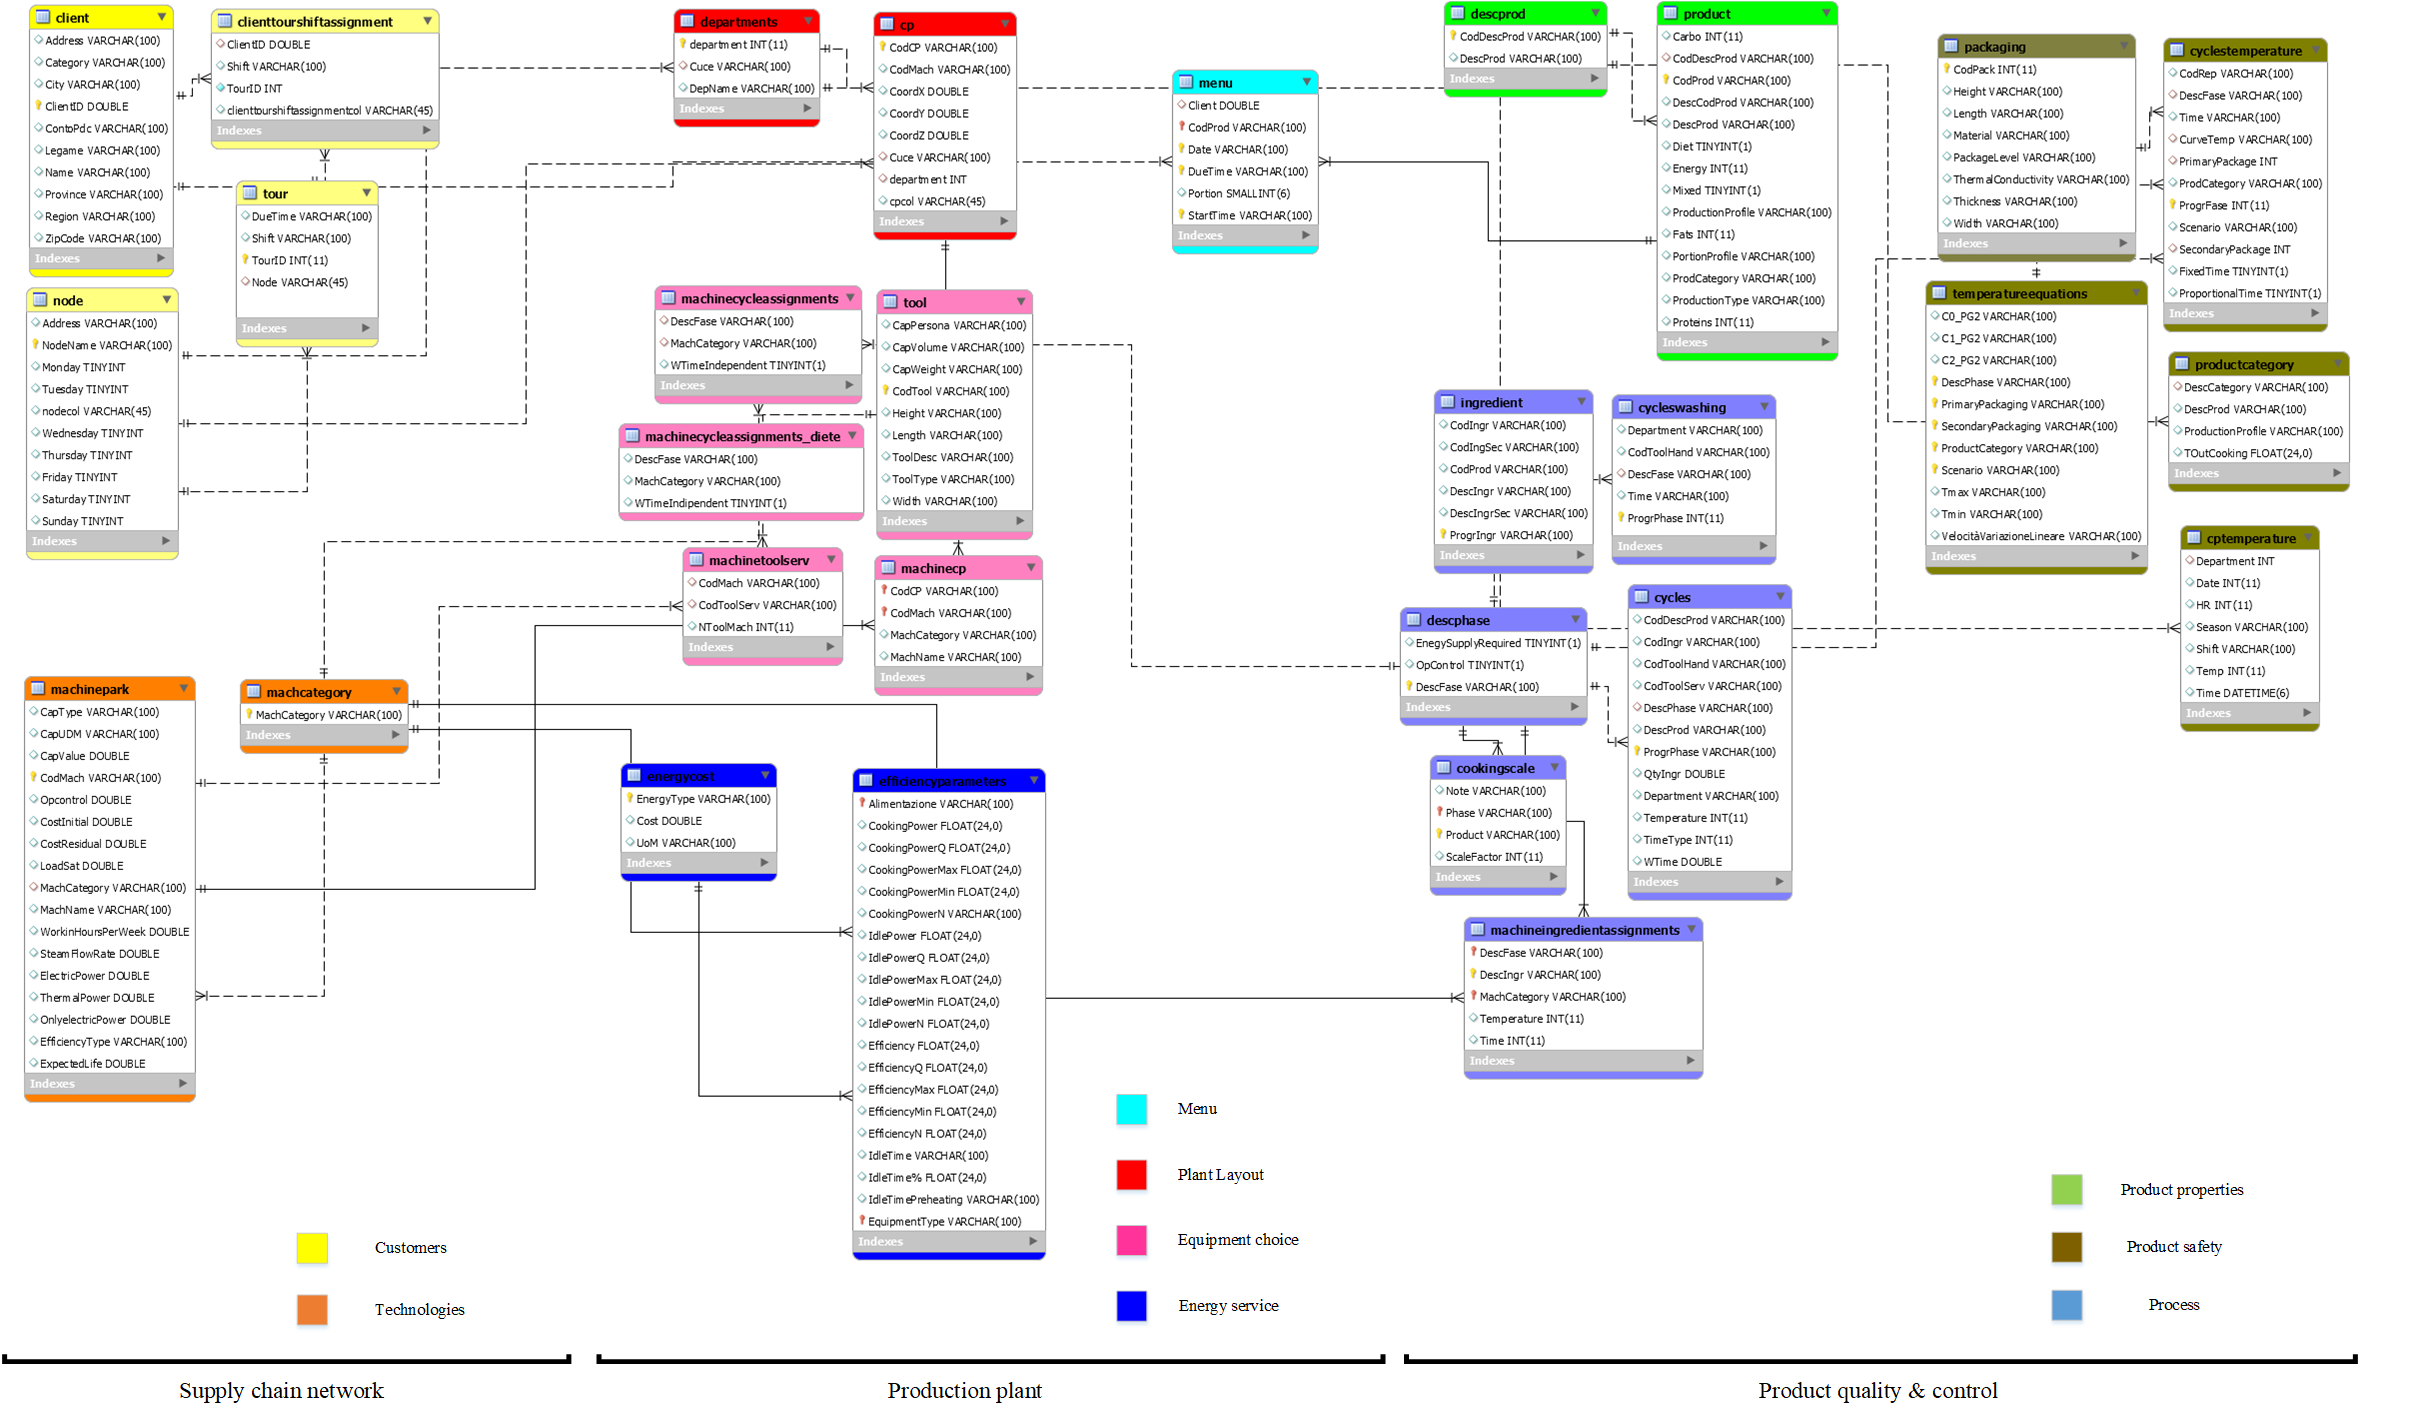
\includegraphics[width=1.6\textwidth]{sectionProduction/diagnosticModels_figures/fig_prod_er_diagram.png}
\captionsetup{type=table}
\caption{ER-model for a production environment in a food catering industry.}
\label{fig_prod_er_diagram}
\end{figure}
\end{landscape}

Figure \ref{fig_prod_er_diagram} remarks the high level of complexity covering a production plant and its modelling. Regardless of the complexity, the bias due to the market niche of the plant leads to the impossibility of a general-purpose model to model entities and processes of any production site. \par

This rigidity may be useful in a production environment to keep track of everything within a robust structure. Nevertheless, it is not a good starting point to analyse data, compare it with different production plants and generalise the results, which is the primary aim of research and this book. For this reason, the following paragraph proposes a different approach using a non-relational structure which removes some bias and allows to generalise some entities for any production system.

\subsection{A Non-relational model for production environments}

This section presents a non-relational data structure able to embed the same information content of the ER model introduced in \ref{secRelationalModelProduction} but able to host any other additional attribute.  In addition, the model has a minimum number of required attributes that enables define a minimum viable model (MVM) enhancing analysis appliable to any production node. This is the natural implementation of the MIP model introduced in section \ref{secInfoFramework}. The model consists of four collections whose data are recorded by the manufacturing execution system (MES). \par

A collection \textit{Part} identifies all the parts $i$ processed within the production plant. The id of the item and the description are required to define the MVM. Other attributes can be stored as well, like:

\begin{itemize}
    \item the size, 
    \item the weight, 
    \item the supplier,
    \item the product family.
\end{itemize}

A collection \textit{Movements} defines the movement function of the MIP model storing information on when a part $i$ enter or leave the production node (or one of its subsystems, as a resource $j$). Attributes timestamp, part id, and quantity are needed for the MVM. Each document can record other attributes as:

\begin{itemize}
    \item the type of package, 
    \item the id of the operator,
    \item the id of the order,
    \item the id of the machine performing a task.
\end{itemize}

A collection \textit{Temmeasurement} store information on on-field time and motion analysis which corrects and complete the measurements of the MES. The id the observation and its duration in seconds define the MVM. \par
A collection \textit{Plant} contains a single document with the information of the production node. The node code is the only attribute necessary to define an MVM. Other attributes can be recorded, like:

\begin{itemize}
    \item the latitude and longitude of the plant,
    \item the address of the plant,
    \item the list of customers served by the plant
    \item the overall productivity of the plant,
    \item the energy absorption of the plant.
\end{itemize}

Figure \ref{fig_MVM_prod} uses the unified modelling language (UML) to represent the MVM of the non-relational structure of a production system.

% INSERT fig_MVM_prod
\begin{figure}[hbt!]
\centering
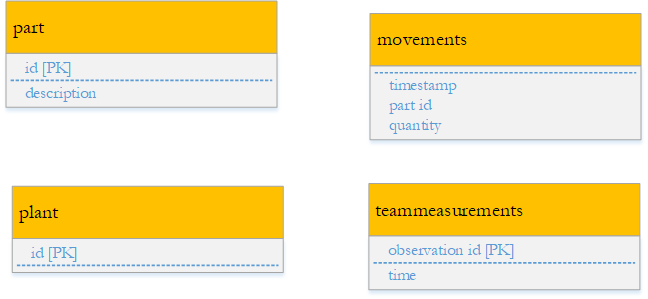
\includegraphics[width=0.8\textwidth]{sectionProduction/diagnosticModels_figures/fig_MVM_prod.png}
\captionsetup{type=figure}
\caption{Diagram in UML notation of the minimum viable model for a non-relational structure of a production system.}
\label{fig_MVM_prod}
\end{figure}


\section{Decision Patterns}
This section introduces the decision patterns (see section \ref{secDecisionPatterns}) analysed in chapters \ref{chapProdControl}, \ref{chapProdPlantDesign} and \ref{chapProdProcessDesign} focusing on the role of analytics to solve production node control, design and process design. Each chapter addresses a family of problems:

\begin{enumerate}
    \item Production control problems, deal with the assessment and improvement of the performance of an existing production plant.
    \item Plant design problems, deal with the design and placement of the physical assets of a production plant;
    \item Process design problems, deal with the definition of the production processes.
\end{enumerate}

Different methodologies allow getting feasible solutions to these problems. Table \ref{tab_problems_prod} illustrates the entities and their definition according to the ontology in Paragraph \ref{secOntology}. 

% INSERT tab_problems_prod
\begin{landscape}
\thispagestyle{empty}
\begin{figure}[hbt!]
\centering
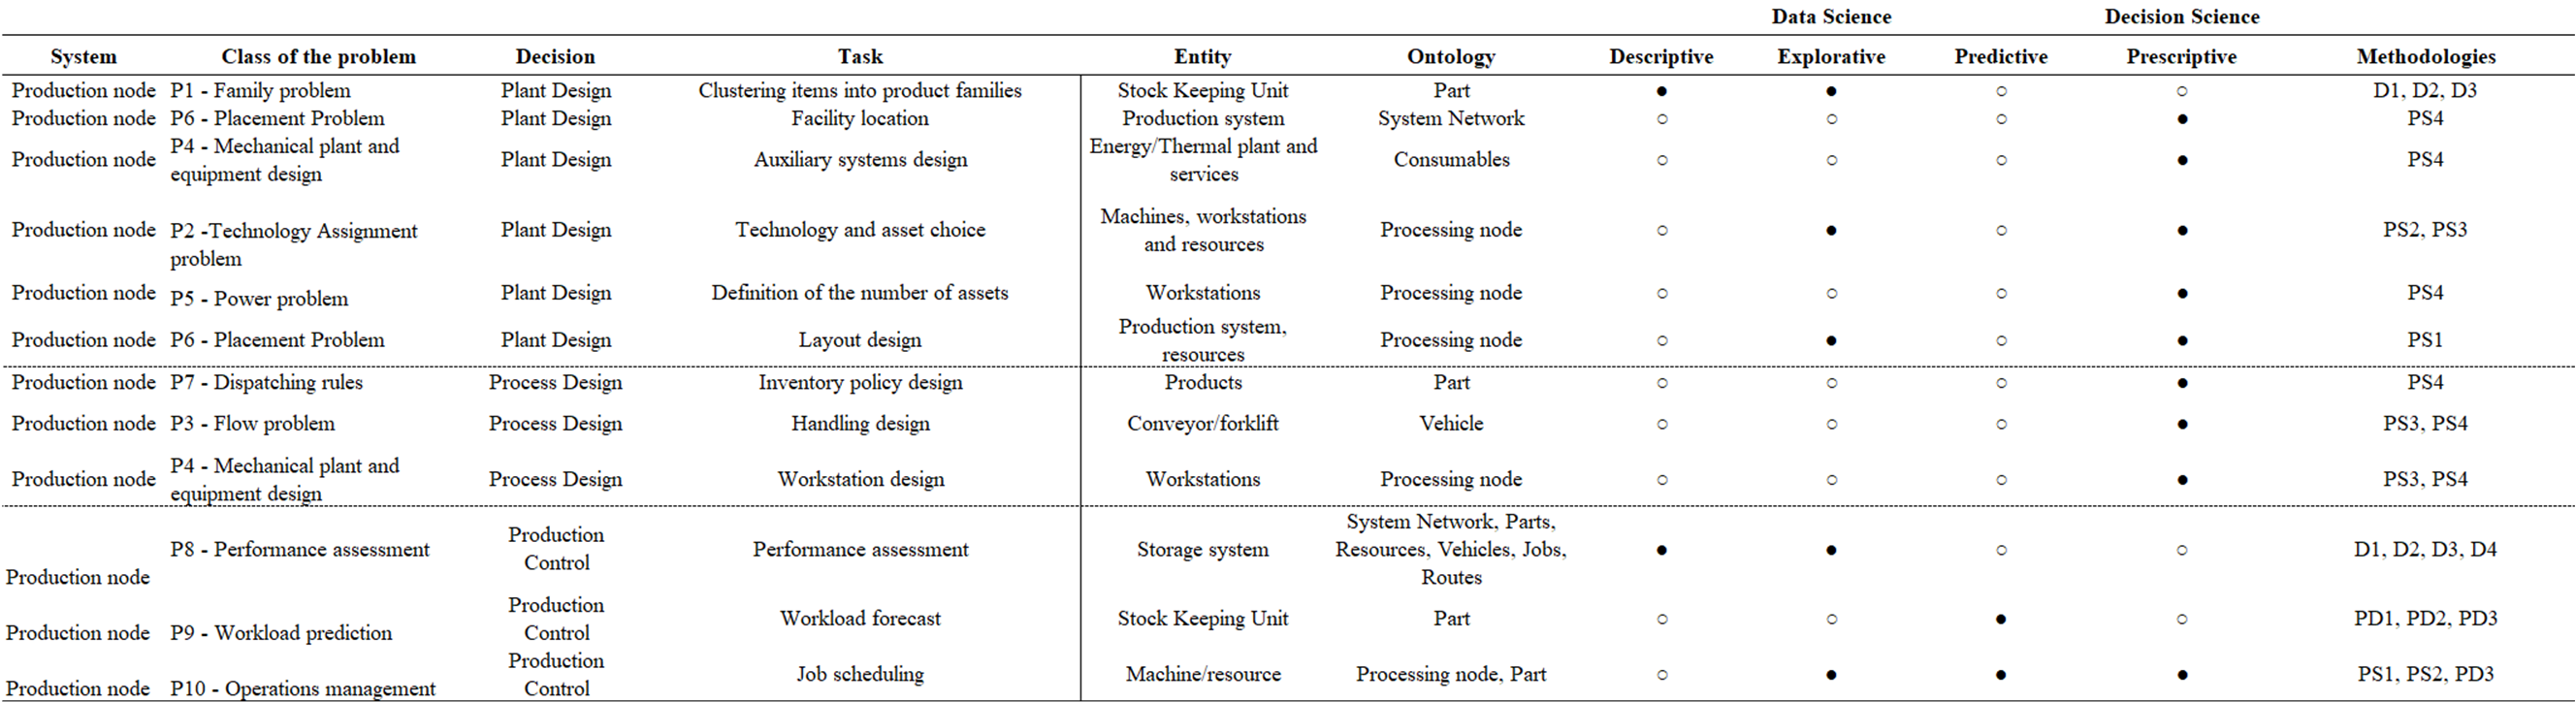
\includegraphics[width=1.5\textwidth]{sectionProduction/diagnosticModels_figures/tab_problems_prod.png}
\captionsetup{type=table}
\caption{Decision problems classification in a production node.}
\label{tab_problems_prod}
\end{figure}
\end{landscape}

Production control involves the following decisions:
\begin{enumerate}
    \item The assessment of the performance of production processes;
    \item The prediction of the market demand and the workload in the future;
    \item The prescription of job scheduling to assign jobs to resources.
\end{enumerate}

Plant design involves the following decisions:
\begin{enumerate}
    \item The definition of homogeneous product families to process and analyse together;
    \item The definition of the location of the physical plant;
    \item The design of the auxiliary system to feed with energy and fluid asset and resources;
    \item The definition of the technology of asset and resources to provide adequate throughput;
    \item The definition of a proper amount of resources identifying a proper production capacity;
    \item The design of the plant layout.

\end{enumerate}

Process design involves the following decisions:
\begin{enumerate}
    \item The definition of an inventory policy and inventory level for parts;
    \item The design of the handling systems to manage the flow of materials within the production plant;
    \item The design of workstation and workbench to smooth production flows, keep order and provide an ergonomic working place to the operators.
\end{enumerate}

